\section{Method}
\paragraph{Overview}
\begin{itemize}
\item compute medial axis transform (MAT)
\item find verts `of high curvature' in the medial axis
\item round the distance measures at those locations to integer multiples of the middle of the range of possible bead widths
\item introduce points on the `arms' of the medial axis connected to the changed verts, around even subdivision of the distance measures
\item connect points to the outline with new fingers
\item introduce new locations on the `fingers' of the medial axis at ideas distances for fingers from non-rounded medial axis verts
\item introduce new locations on the fingers at regular intervals for medial axis verts with rounded distance measures
\item connect all locations to form the inset polygons and polylines
\end{itemize}


\subsection{Straight Skeleton or Medial Axis?}
Medial Axis!
Medial axis is stable against small perturbations in the input polygon!
Concave corners are handled irrespective of how many vertices are in a corner.


$\to$ approximate parabolas for simpler processing!

This approximation leads to even spacing,
while a derived formula seems to produce different results:

See \url{/home/t.kuipers/Documents/PhD/Variable_Width_project/pathplanning preliminaries/medial_axis_parabolas.svg}

\Cref{medial_axis_parabolas}

\hl{But the uneven spacing figure looks like its evenly spaced in the direction orthogonal to the toolpath itself!}


\begin{figure}
\begin{subfigure}{0.45\columnwidth}
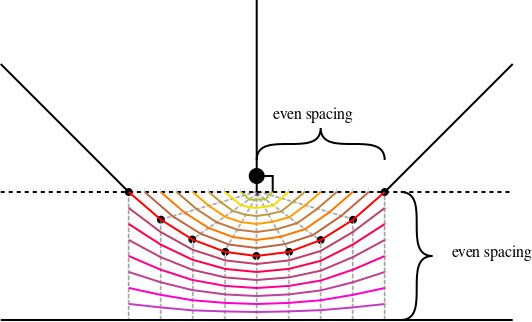
\includegraphics[width=\columnwidth]{sources/method/medial_axis_even_spacing.jpg}
\end{subfigure}
\begin{subfigure}{0.45\columnwidth}
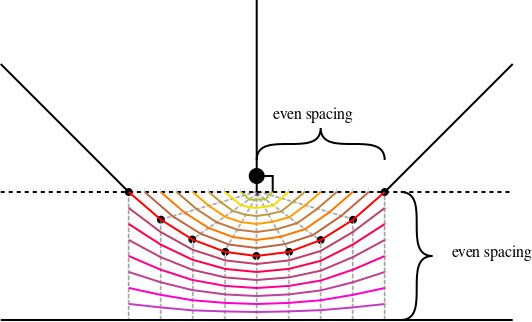
\includegraphics[width=\columnwidth]{sources/method/medial_axis_even_spacing.jpg}
\end{subfigure}
\caption{The equidistant points between a vert and a line form a parabola. There are different methods for generating toolpaths which are in between the medial axis and the outline.}
\label{medial_axis_parabolas}
\end{figure}




\subsection{Angle of fingers introduced on the skeleton}
\Cref{finger_angles}
Cannot be optimized.
Always has to be orthogonal to the polygon segment.
Otherwise the algorithm isn’t stable w.r.t. extra vertices.

\begin{figure}
\begin{subfigure}{0.45\columnwidth}
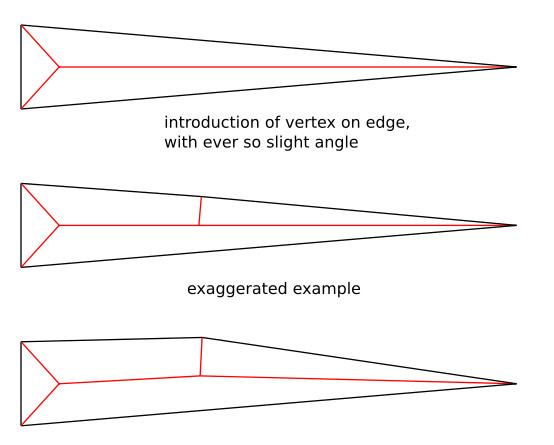
\includegraphics[width=\columnwidth]{sources/method/finger_angles.jpg}
\end{subfigure}
\begin{subfigure}{0.45\columnwidth}
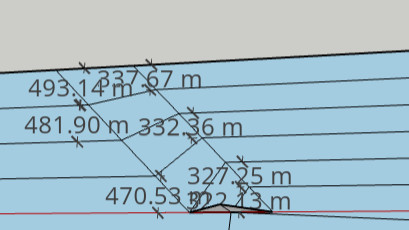
\includegraphics[width=\columnwidth]{sources/method/finger_angles_2.jpg}
\end{subfigure}
\caption{Figner angles should always be orthogonal}
\label{finger_angles}
\end{figure}



\subsection{Single bead segments}
\Cref{single_bead_strategy}
Could be printed from polygon and return to polygon over same segment without extruding

How to deal with single beads connecting two polys?
: Print 1st poly $\to$ print single bead $\to$ print 2nd poly $\to$ travel over single bead $\to$ print 1st poly

How to deal with three-way intersection single beads?
: Cut up in 1 single bead connecting two polys and 1 normal single bead only connected to one poly

\begin{figure}
\begin{subfigure}{0.45\columnwidth}
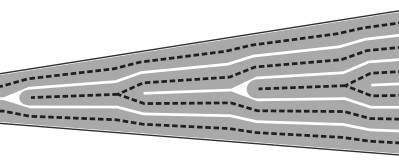
\includegraphics[width=\columnwidth]{sources/method/single_bead_strategy.jpg}
\end{subfigure}
\begin{subfigure}{0.45\columnwidth}
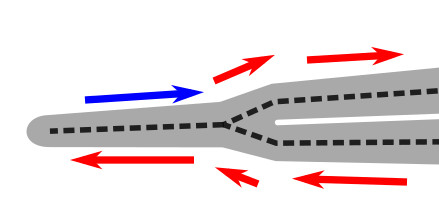
\includegraphics[width=\columnwidth]{sources/method/single_bead_strategy_order.jpg}
\end{subfigure}
\caption{We can do single-bead segments. Blue is travel move.}
\label{single_bead_strategy}
\end{figure}


\subsection{When to introduce fingers?}
Depends on the angle between the poly segments

When to introduce joints rather than using existing joints? When round joint distances to integer multiples of the nozzle size rather than introducing a new joint?

\paragraph{We could introduce bones implicitly.}
Instead of changing the straight skeleton and introducing bones,
we can simply introduce new vertices on the polygon and generate a new straight skeleton.



\subsection{Where to add fingers?}
\Cref{rounded_dist_measures}
Based on unrounded distance measures.
Otherwise we don’t get the switch to twice the bead width
Moreover, the algorithm wouldn’t be stable: the locations where bones would get introduces would depend on where the other joints are, instead of on the distance measure.

\hl{But what does this mean?
When should I round distances to integer multiples?!}

\begin{figure}
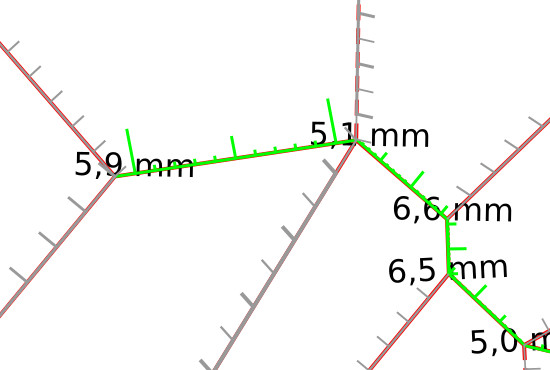
\includegraphics[width=\columnwidth]{sources/method/rounded_dist_measures.jpg}
\caption{Distance measure rounding}
\label{rounded_dist_measures}
\end{figure}


























